\documentclass{beamer}
\usepackage[utf8]{inputenc}
\usepackage[T1]{fontenc}
\usepackage[english]{babel}
\usepackage{lmodern}
\usepackage{amsmath}
\usepackage{amssymb}
\usepackage{amsthm}
\usepackage[superscript]{cite}
\usepackage{nicefrac}
\usepackage{upgreek}
\usepackage{stmaryrd}
\usepackage{tikz}
\usepackage{graphicx}
\usepackage{qtree}
\usepackage{dsfont}
\usepackage{eurosym}
\usepackage{tabulary}
\usepackage{setspace}
% \usepackage[colorlinks=true,linkcolor=blue]{hyperref}				% Blaue Links sehen meiner Ansicht nach besser aus als die rot umrandeten Verweise

\usetheme{Madrid}				% Verwende Goettingen für TOC auf jeder Seite, Madrid ohne Navigation

% Kommandos, Operatoren, etc.
\newcommand{\abs}[1]{\lvert#1\rvert}
\newcommand{\norm}[1]{\lVert#1\rVert}
\DeclareMathOperator{\thetafunc}{\uptheta}

% ENDE PRÄAMBEL

\AtBeginSection[]{
	\begin{frame}
		\vfill
		\centering
		\begin{beamercolorbox}[sep=8pt,center,shadow=true,rounded=true]{title}
			\usebeamerfont{title}\insertsectionhead\par%
		\end{beamercolorbox}
		\vfill
	\end{frame}
}

\author{Dominik Blank}
\title{ROI Testing}
\institute{Georg-August-Universität Göttingen}

\setlength{\parindent}{0pt}
\allowdisplaybreaks

\begin{document}

\begin{frame}
	\maketitle
\end{frame}

\begin{frame}
	\tableofcontents
\end{frame}

\section{ROI Testing}

\subsection{The statistical model}

\begin{frame}
	Let $M, N \in \mathbb{N}$ and $\Omega = \left\{ 0, \dots, M-1 \right\} \times  \left\{ 0, \dots, N-1 \right\}$. Assume we are given data
	\begin{equation*}\label{model}
		F(i, j) = c + V(i, j) + \varepsilon_{i, j}
	\end{equation*}
	\begin{itemize}
		\item $(i, j) \in \Omega$
		\item $c \in \mathbb{R}$ is constant
		\item $V(i, j) \in \{ 0, \pm c \}$
		\item $\varepsilon_{m, n} \sim \mathcal{N}(0, \sigma^2)$ i.i.d. normal distributed random variables
	\end{itemize}
	
	Assumption 1: The image $F$ contains a rectangular region of interest.
	Assumption 2: The ROI has a checkerboard pattern.
\end{frame}

\begin{frame}
	\begin{figure}
		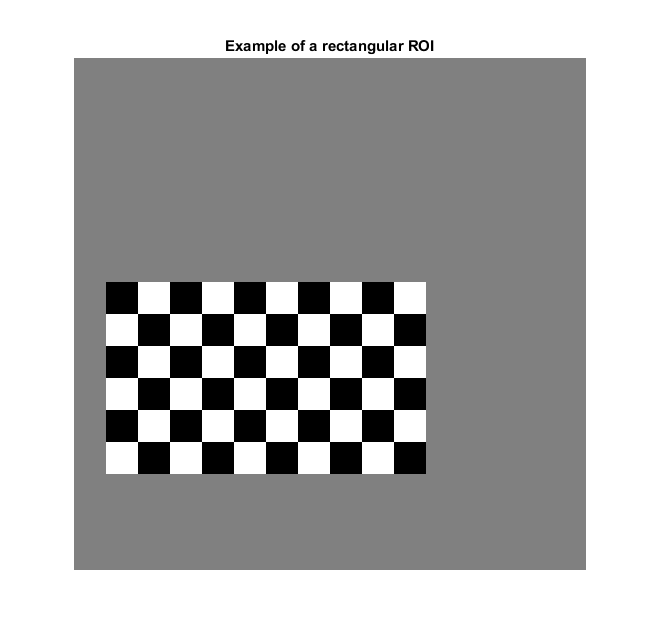
\includegraphics[width=0.6\linewidth]{Testing/ROI}
		\caption[ROI]{Example of a possible region of interest. ($M = 16$, $N = 16$)}
		\label{fig:ROI}
	\end{figure}
\end{frame}

\begin{frame}
	\begin{figure}
		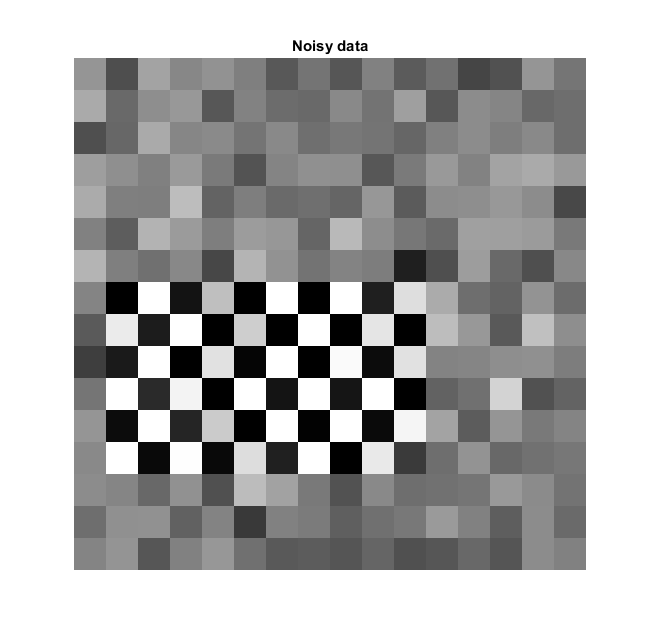
\includegraphics[width=0.6\linewidth]{Testing/ROI_noisy}
		\caption[Noisy ROI]{Same region of interest with noise added. ($\sigma = 30$)}
		\label{fig:ROI_noisy}
	\end{figure}
\end{frame}

\subsection{Testing for the ROI}

\begin{frame}
	\begin{beamercolorbox}[sep=8pt,center,shadow=true,rounded=true]{title}
		Goal: Construct a statistical test for the region of interest.
	\end{beamercolorbox}
\end{frame}

\subsubsection{The statistical test}

\begin{frame}
	For each pixel $(i, j) \in \Omega$ we define four non-observable and four observable values
	\begin{align*}
		\textrm{non-observable}
		&\begin{cases}
			D_1^\pm(i, j) = V(i \pm 1, j) - V(i, j) \\
			D_2^\pm(i, j) = V(i, j \pm 1) - V(i, j) \\
		\end{cases} \\
		\textrm{observable}
		&\begin{cases}
			\tilde{D}_1^\pm(i, j) = F(i \pm 1, j) - F(i, j) \\
			\tilde{D}_2^\pm(i, j) = F(i, j \pm 1) - F(i, j)
		\end{cases}
	\end{align*}
	and combine them to new values
	\begin{align*}\label{d}
		D^\pm(i, j) &= \sqrt{D_1^\pm(i, j)^2 + D_2^\pm(i, j)^2} \\
		\tilde{D}^\pm(i, j) &= \sqrt{\tilde{D}_1^\pm(i, j)^2 + \tilde{D}_2^\pm(i, j)^2}
	\end{align*}
\end{frame}

\begin{frame}
	\begin{figure}
		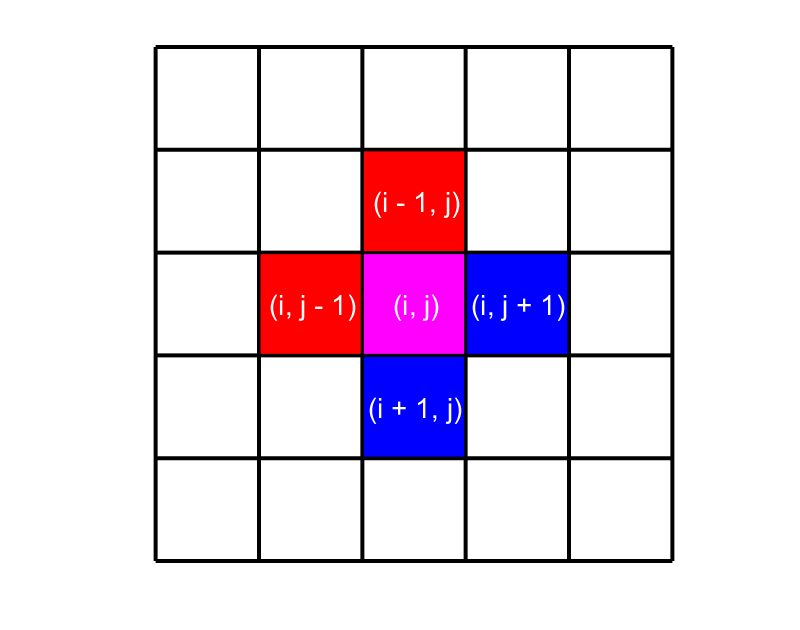
\includegraphics[width=0.6\linewidth]{Testing/TestStatistic}
		\caption[Test Statistic]{Pixel $(i, j)$ with its neigbour pixels. The blue neighbours are used to calculate $\tilde{D}^+(i, j)$ and the red neighbours are used to calculate $\tilde{D}^-(i, j)$. The purple pixel is used for both $\tilde{D}^+(i, j)$ and $\tilde{D}^-(i, j)$.}
		\label{fig:TestStatistic}
	\end{figure}
\end{frame}

\begin{frame}
	We now test the null hypothesis $$H_0 : \min\{ D^+(i, j), D^-(i, j) \} = 0$$ against the alternative hypothesis $$H_1 : \min\{ D^+(i, j), D^-(i, j) \} > 0$$ using the test statistic $$T = \min \{ \tilde{D}^+(i, j), \tilde{D}^-(i, j) \}$$
\end{frame}

\subsubsection{Statistical significance}

\begin{frame}
	\begin{beamercolorbox}[sep=8pt,center,shadow=true,rounded=true]{title}
		Question: How do we determine the distribution of the test statistic $T$ under the null hypothesis $H_0$?
	\end{beamercolorbox}
\end{frame}

\begin{frame}
	We observe that
	\begin{equation*}
		\mathbb{P}(T \geq t \mid H_0) \leq \mathbb{P}(\tilde{D}^\pm(i, j) \geq t \mid D^\pm(i, j) = 0)
	\end{equation*}
	Thus, if we can find a threshold $t_\alpha$, s.t.
	\begin{equation*}
		\mathbb{P}(\tilde{D}^\pm(i, j) \geq t_\alpha \mid D^\pm(i, j) = 0) \leq \alpha
	\end{equation*}
	for a given $\alpha$, we have ensured a statistical significance of $\alpha$.
\end{frame}

\begin{frame}
	Let $\varepsilon_{i, j}$ be fixed. Then
	\begin{align*}
		&\mathbb{P}(\tilde{D}^\pm(i, j) \leq t \mid D^\pm(i, j) = 0) \\
		&= \mathbb{P}\left( (\varepsilon_{i \pm 1, j} - \varepsilon_{i, j})^2 + (\varepsilon_{i, j \pm 1} - \varepsilon_{i, j})^2 \leq t^2 \right) \\
		&= \mathbb{P}\left( \sqrt{\left( \frac{X_1}{\sigma} \right)^2 + \left( \frac{X_2}{\sigma} \right)^2} \leq \frac{t}{\sigma} \right)
	\end{align*}
	with $X_1 = \varepsilon_{i \pm 1, j} - \varepsilon_{i, j}$, $X_2 = \varepsilon_{i, j \pm 1} - \varepsilon_{i, j}$ and $Y = \varepsilon_{i, j}$. Then
	\begin{align*}
		X_1 &\sim \mathcal{N}(- Y, \sigma^2) \\
		X_2 &\sim \mathcal{N}(- Y, \sigma^2) \\
		Y &\sim \mathcal{N}(0, \sigma^2)
	\end{align*}
	
	Then we can see, that the square root inside has non-central chi distribution with two degrees of freedom and non-centrality parameter
	\begin{equation*}
		\lambda = \frac{\sqrt{2} \abs{Y}}{\sigma}
	\end{equation*}
\end{frame}

\begin{frame}
	So far we assumed $\varepsilon_{i, j}$ to be fixed, but it actually is a random variable itself with normal distribution: $\varepsilon_{i, j} \sim \mathcal{N}(0, \sigma^2)$. Thus, we have a compound probability distribution:
	\begin{align*}
		&\mathbb{P}(\tilde{D}^\pm(i, j) \leq t \mid D^\pm(i, j) = 0) \\
		&= \int_0^\frac{t}{\sigma} \int_0^\infty \underbrace{x \exp \left( - \frac{x^2}{2} - \frac{y^2}{\sigma^2} \right) I_0 \left( \frac{\sqrt{2} y}{\sigma} x \right)}_{\textrm{pdf of} \ \chi_2 \left( \frac{\sqrt{2} y}{\sigma} \right) \ \textrm{for fixed} \ y} \underbrace{\frac{2}{\sqrt{2 \pi \sigma^2}} \exp \left( - \frac{y^2}{2 \sigma^2} \right)}_{\textrm{pdf of absolute value of} \ \mathcal{N}(0, \sigma^2)} dy dx \\
		&= \frac{1}{\sqrt{3}} \left( \frac{3}{2} - \frac{3}{2} \exp \left( - \frac{t^2}{3 \sigma^2} \right) I_0 \left( \frac{t^2}{6 \sigma^2} \right) \right) - \sqrt{3} \\
		&- \frac{2 - \sqrt{3}}{2} Q_1 \left( \frac{2 - \sqrt{3}}{6} \sqrt{\frac{t}{\sigma}}, \frac{2 + \sqrt{3}}{6} \sqrt{\frac{t}{\sigma}} \right) \\
		&+ \frac{2 + \sqrt{3}}{2} Q_1 \left( \frac{2 + \sqrt{3}}{6} \sqrt{\frac{t}{\sigma}}, \frac{2 - \sqrt{3}}{6} \sqrt{\frac{t}{\sigma}} \right)
	\end{align*}
\end{frame}

\begin{frame}
	With an easy program the threshold for a given $\alpha$ can be calculated. As can be seen from the CDF, it is enough to calculate the threshold $t_\alpha$ for $\sigma = 1$ and multiply the outcome by $\sigma$.
	\begin{figure}
		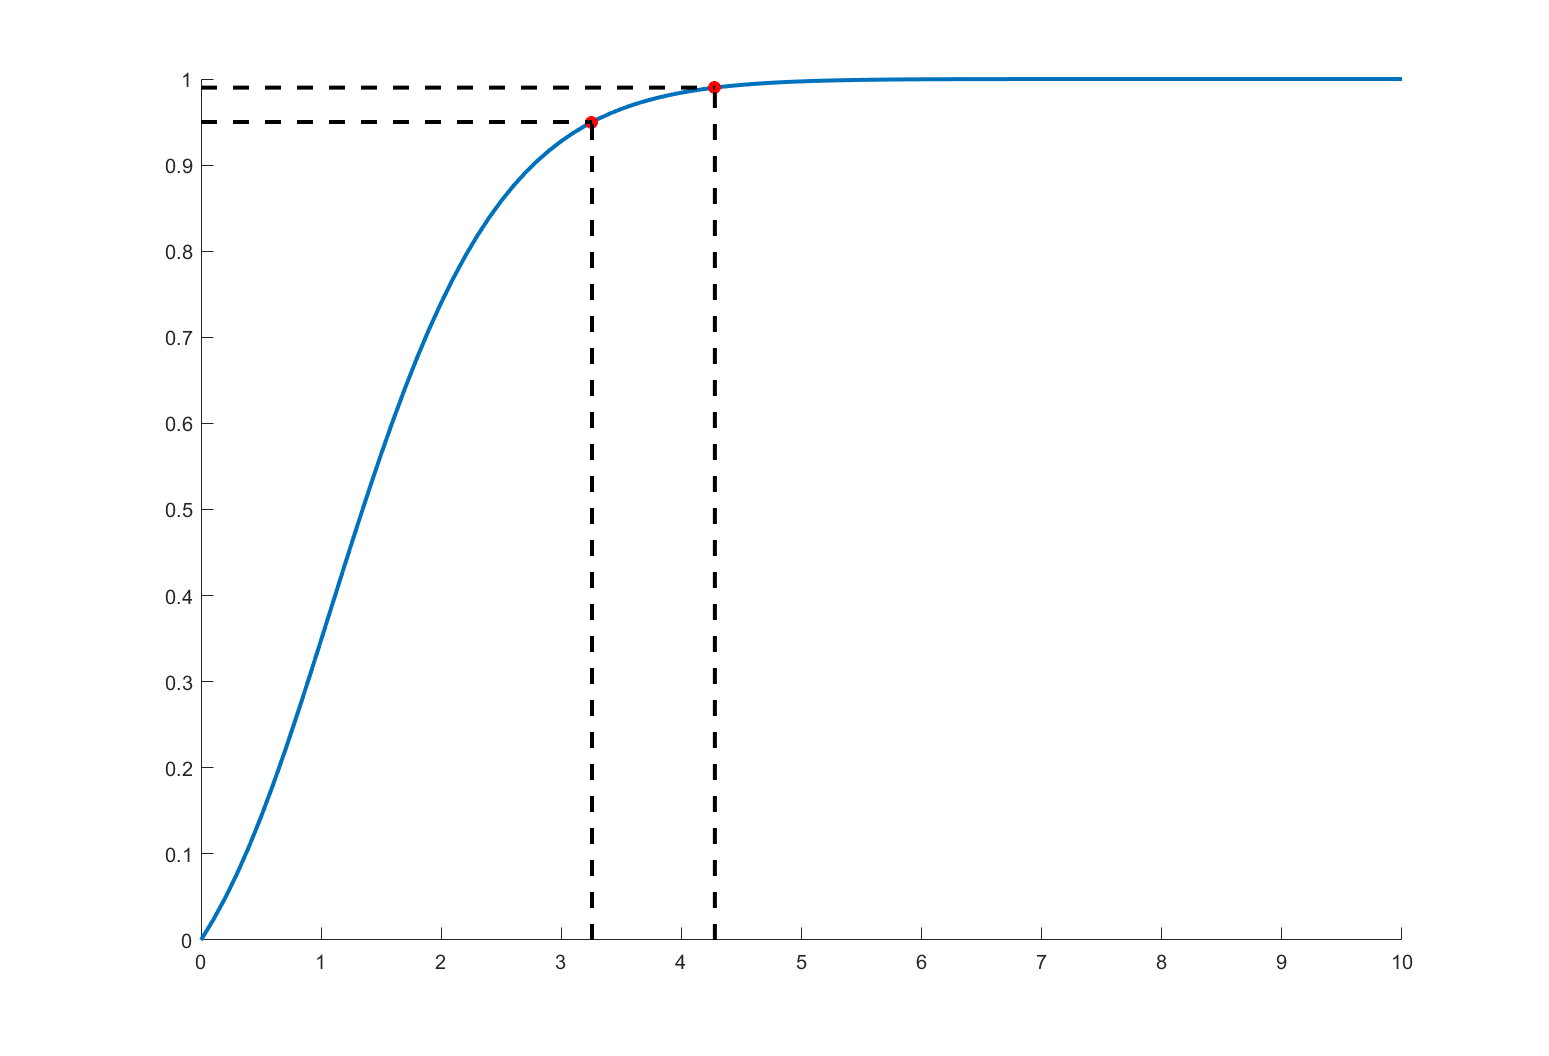
\includegraphics[width=0.6\linewidth]{Testing/CDF}
		\caption[CDF]{Cumulative distribution function of $\mathbb{P}(\tilde{D}^\pm(i, j) \leq t \mid D^\pm(i, j) = 0)$ with thresholds for $\alpha = 0.05$ and $\alpha = 0.01$. ($t_{0.05} = 3.2554$, $t_{0.01} = 4.2791$, $\sigma = 1$)}
		\label{fig:CDF}
	\end{figure}
\end{frame}

\subsubsection{Power of the test}

\begin{frame}
	We are also interested in bounds for the power of this test.
	
	Using results and notations from the previous sections, we get the upper bound
	\begin{equation*}
		1 - \beta = \mathbb{P}(T \geq t \mid H_1) \leq \mathbb{P}(\tilde{D}^+(i, j) \geq t \mid D^+(i, j) = \sqrt{8} c)
	\end{equation*}
	
	On the other hand, we get the lower bound
	\begin{equation*}
		1 - \beta = \mathbb{P}(T \geq t \mid H_1) \geq 2 \cdot \mathbb{P}(\tilde{D}^+(i, j) \geq t \mid D^+(i, j) = c) - 1
	\end{equation*}
	
	Thus we can conclude, that
	\begin{equation*}
		1 - \beta \geq \max \left\{ 2 \cdot \mathbb{P}(\tilde{D}^+(i, j) \geq t \mid D^+(i, j) = c) - 1, 0 \right\}
	\end{equation*}
\end{frame}

\subsubsection{Numerical results}

\begin{frame}
	By simulating the probabilities $\mathbb{P}(\tilde{D}^+(i, j) \geq t \mid D^+(i, j) = \sqrt{8} c)$ and $\mathbb{P}(\tilde{D}^+(i, j) \geq t \mid D^+(i, j) = c)$, we can get empirical bounds for the power of our test.
	
	We have the following relation
	\begin{alignat*}{2}
		D^+(i, j) &= \sqrt{8} c &&\Rightarrow D_1^+(i, j) = D_2^+(i, j) = 2 c \\
		D^+(i, j) &= c &&\Rightarrow D_1^+(i, j) = D_2^+(i, j) = c
	\end{alignat*}
	
	Simulation of the probabilities can be done by following these steps:
	\begin{itemize}
		\item Simulate $\mathcal{N}(0, \sigma^2)$ random variables.
		\item Calculate $\tilde{D}^+(i, j)$ conditioned on either $D^+(i, j) = \sqrt{8} c$ or $D^+(i, j) = c$.
		\item Count proportion of simulations where $D^+(i, j) \geq t_\alpha \sigma$.
	\end{itemize}
\end{frame}

\begin{frame}
	In the case of a grayscale image, we assume $c = 127.5$. For $t_{0.05} = 3.2554$ and $10.000.000$ simulations of the noise terms, we get the following empirical bounds dependent on the standard deviation $\sigma$.
	
	\begin{figure}[h]
		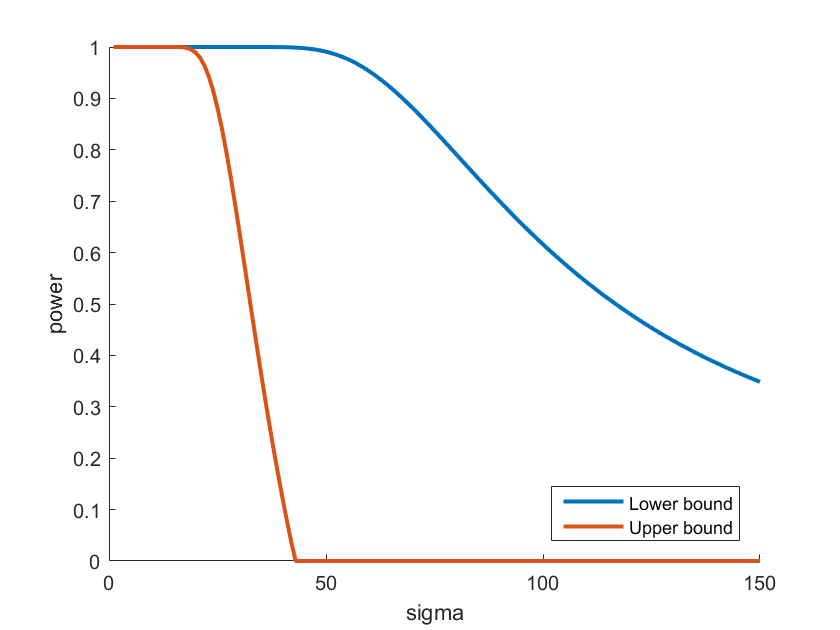
\includegraphics[width=0.6\linewidth]{Testing/SimulatedPower}
		\caption[Simulated power bounds]{For $\alpha = 0.05$ this graph shows the lower and upper bounds for the power of the test for $\sigma \in \{ 1, 2, \dots, 150 \}$.}
		\label{fig:SimulatedPowerBounds}
	\end{figure}
\end{frame}

\begin{frame}
	Since $D^\pm(i, j)$ is the sum of dependent squared normal distributed random variables, it is not a simple Chi distributed random variable. If it were, we would get
	\begin{equation*}
		1 - \beta \in \left[ \max \left\{ 2 \cdot Q_1 \left( \frac{c}{\sqrt{2} \sigma}, \frac{t}{\sqrt{2} \sigma} \right) - 1, 0 \right\}, Q_1 \left( \frac{2 c}{\sigma}, \frac{t}{\sqrt{2} \sigma} \right) \right]
	\end{equation*}
\end{frame}

\begin{frame}
	In the independent case we would take $t = 2 \sigma \sqrt{- \log(\alpha)} \approx 3.3616 \sigma$ and get the following bounds for the power dependent on $\sigma$. It is remarkable, how similar these bounds are to the empirical bounds.
	
	\begin{figure}[h]
		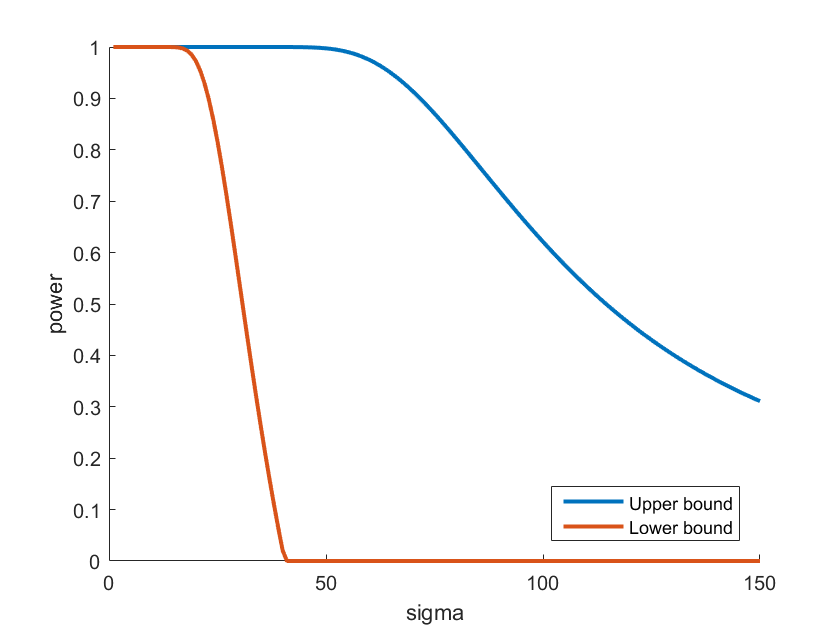
\includegraphics[width=0.6\linewidth]{Testing/TheoreticalPower}
		\caption[Theoretical power bounds]{For $\alpha = 0.05$ this graph shows the lower and upper bounds for the power of the test for $\sigma \in \{ 1, 2, \dots, 150 \}$, if the terms of $\tilde{D}^\pm(i, j)$ were independent.}
		\label{fig:TheoreticalPowerBounds}
	\end{figure}
\end{frame}

\section{Morphological operations}

\subsection{Opening and closing}

\begin{frame}
	Reminder: We always consider structuring elements with odd side length.
	
	\begin{figure}[h]
		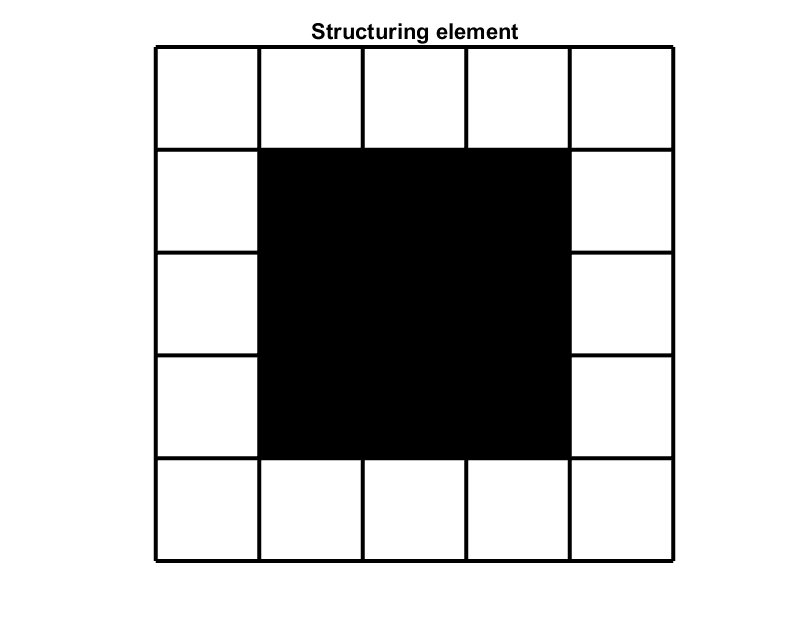
\includegraphics[width=0.6\linewidth]{Morphology/StructuringElement}
		\caption[Structuring Element]{A $3 \times 3$ structuring element.}
		\label{fig:structuringelement}
	\end{figure}
\end{frame}

\begin{frame}
	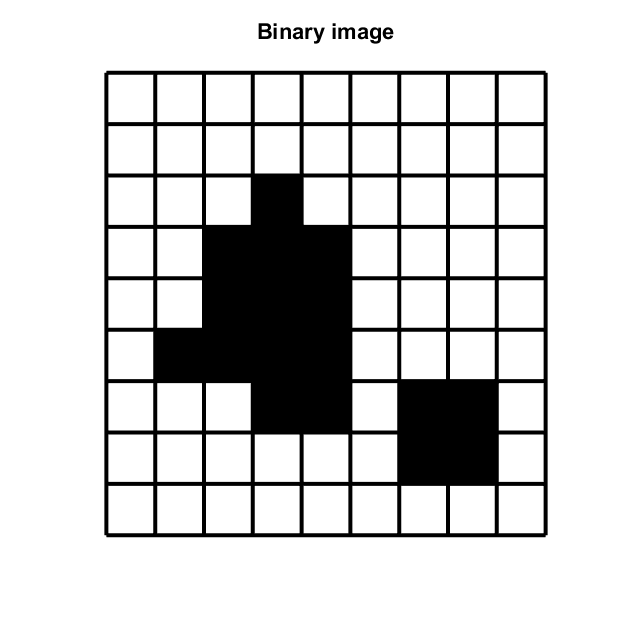
\includegraphics[width=0.3\linewidth]{Morphology/OpeningBefore}
	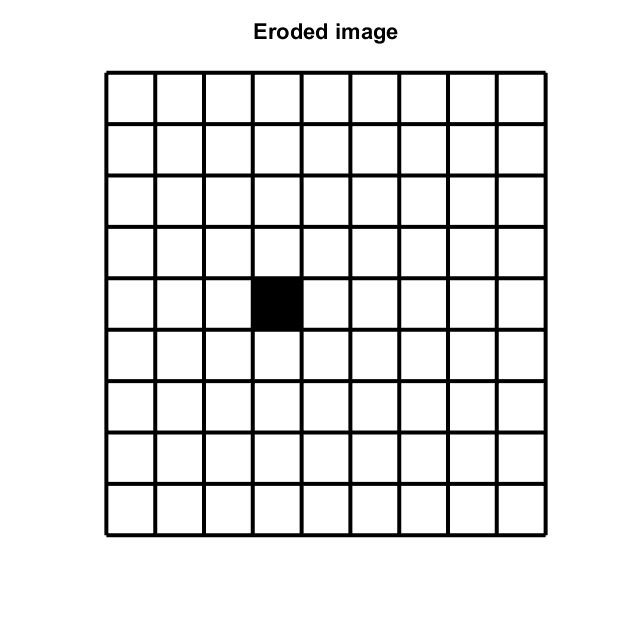
\includegraphics[width=0.3\linewidth]{Morphology/OpeningErode}
	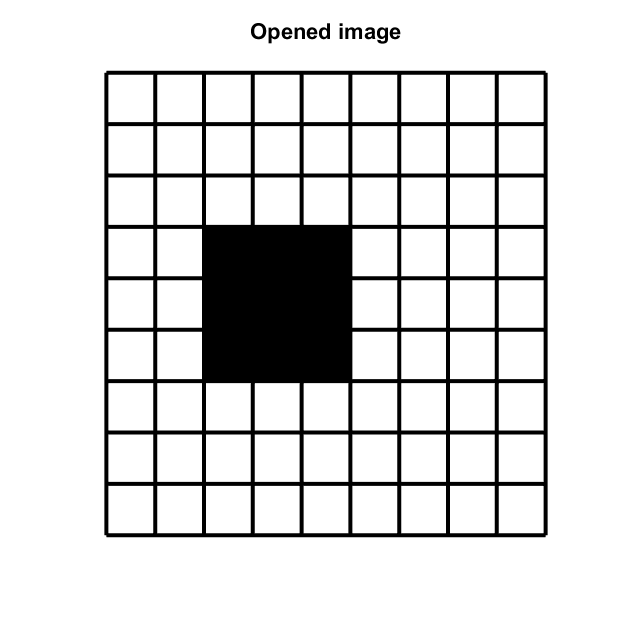
\includegraphics[width=0.3\linewidth]{Morphology/OpeningOpen}
	
	Example of a binary image (black boxes represent 1). The second image is the erosion of the image by a $3 \times 3$ structuring element. The third image is the dilation of the erosion, i.e. the opening of the image.
\end{frame}

\begin{frame}
	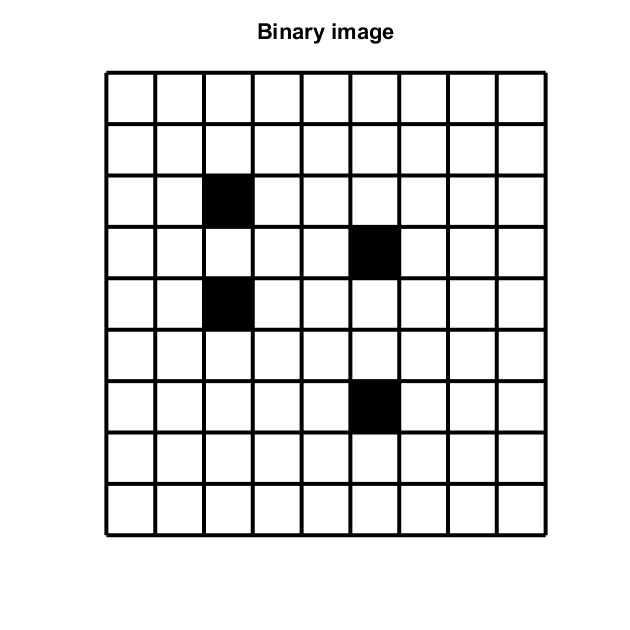
\includegraphics[width=0.3\linewidth]{Morphology/ClosingBefore}
	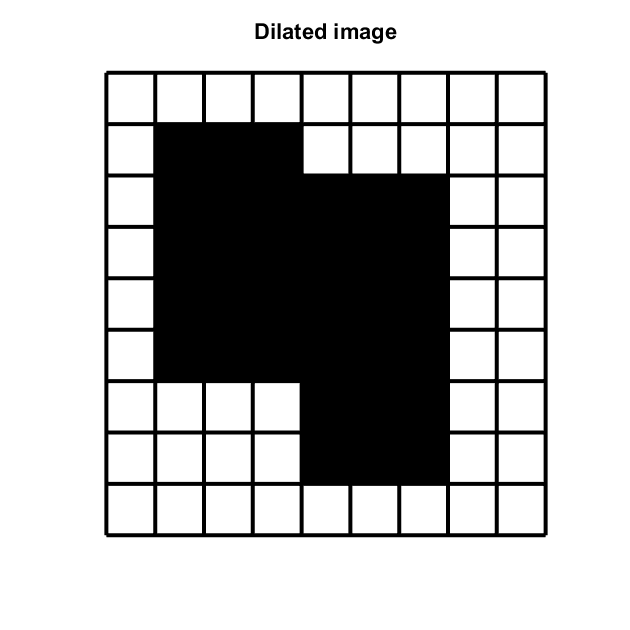
\includegraphics[width=0.3\linewidth]{Morphology/ClosingDilate}
	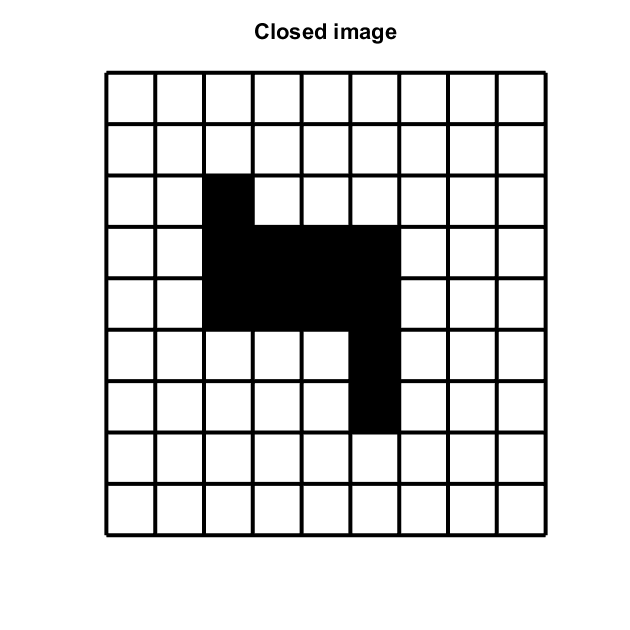
\includegraphics[width=0.3\linewidth]{Morphology/ClosingClosed}
	
	Example of a binary image (black boxes represent 1). The second image is the dilation of the image by a $3 \times 3$ structuring element. The third image is the erosion of the dilation, i.e. the closing of the image.
\end{frame}

\subsection{Hypothesis testing and opening}

\begin{frame}
	\begin{beamercolorbox}[sep=8pt,center,shadow=true,rounded=true]{title}
		Question: What is the effect of opening and closing on statistical significance and power?
	\end{beamercolorbox}
\end{frame}

\begin{frame}
	We will now take a look at the effect of opening on the significance level.
	
	\begin{theorem}
		Let $F$ be an image that contains a rectangular ROI. Assume that we are given a binarized image $F_{bin}$ with
		\begin{equation*}
			\mathbb{P}(F_{bin}(i, j) = 1 \mid H_0(i, j)) \leq \alpha
		\end{equation*}
		where $H_0(i, j)$ denotes the null hypothesis for the pixel $(i, j)$.
		
		Let $k \in \mathbb{N}$ be odd and $B$ be a square structuring element with side length $k$. Then the following inequality holds:
		\begin{equation*}
			\mathbb{P}((F_{bin} \circ B)(i, j) = 1 \mid H_0(i, j)) \leq k \alpha^\frac{k - 1}{2}
		\end{equation*}
	\end{theorem}
\end{frame}

\begin{frame}
	Outline of the proof:
	\begin{itemize}
		\item Note, that if $H_0$ is true for $(i, j)$, then $H_0$ is true for a whole row or column in the image.
		\item With our notation from the test, this means, that $D^+ = 0$ or $D^+ = 0$ for the whole row/column.
		\item If we only take every second pixel in the row/column, they will be independent, which yields the exponent $\frac{k - 1}{2}$.
	\end{itemize}
\end{frame}

\begin{frame}
	\begin{figure}[h]
		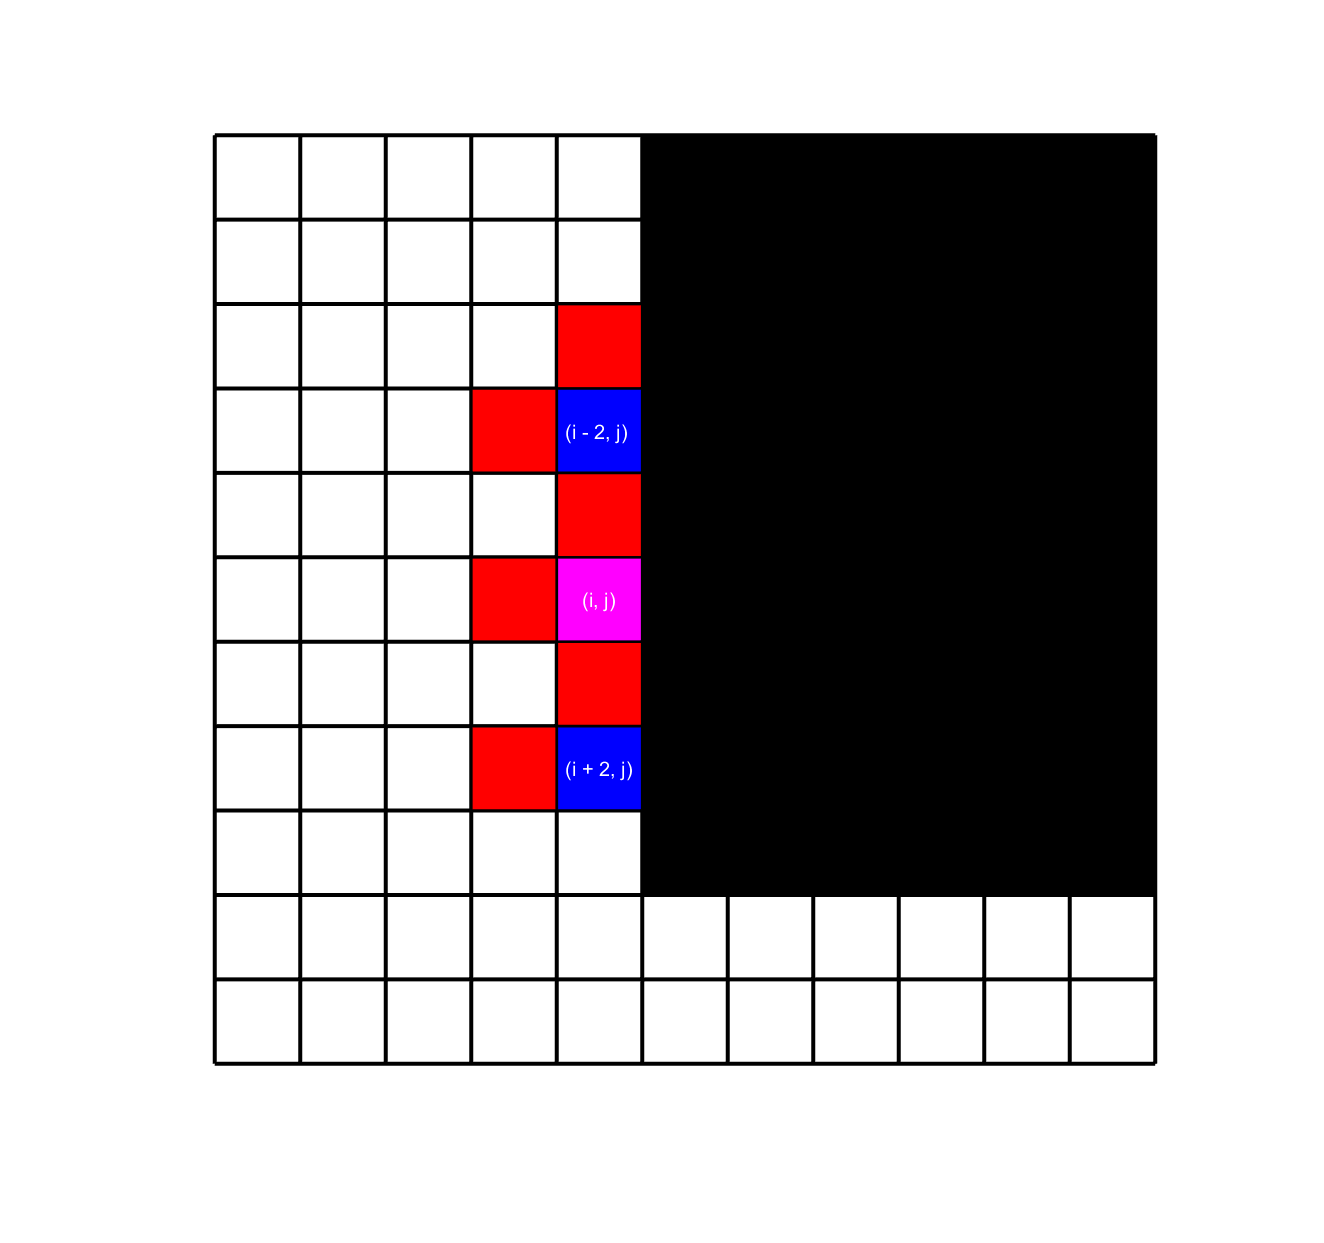
\includegraphics[width=0.6\linewidth]{Morphology/IndependentPoints}
		\caption[Independent points]{If we consider only every second pixel in the column, these will be independent.}
		\label{fig:IndependentPoints}
	\end{figure}
\end{frame}

\subsection{Hypothesis testing and closing}

\begin{frame}
	We will also take a look at the effect of closing on the significance level.
	
	\begin{theorem}
		Let $F$ be an image that contains a rectangular ROI. Assume that we are given a binarized image $F_{bin}$ with
		\begin{equation*}
			\mathbb{P}(F_{bin}(i, j) = 1 \mid H_0(i, j)) \leq \alpha
		\end{equation*}
		where $H_0(i, j)$ denotes the null hypothesis for the pixel $(i, j)$.
		
		Let $k \in \mathbb{N}$ be odd and $B$ be a square structuring element with side length $k$. Then the following inequality holds:
		\begin{equation*}
			\mathbb{P}((F_{bin} \bullet B)(i, j) = 1 \mid H_0(i, j)) \leq k^2 \alpha
		\end{equation*}
	\end{theorem}
\end{frame}

\begin{frame}
	Outline of the proof:
	\begin{itemize}
		\item Note, that if $H_0$ is true for $(i, j)$, then there exists a square with side length $k$, such that $H_0$ is true for every pixel inside that square.
		\item The square has $k^2$ pixels and for each pixel the null hypothesis holds, so each pixel has probability $\leq \alpha$ for a type I error.
	\end{itemize}
\end{frame}

\begin{frame}
	Putting both results together, one gets
	\begin{equation*}
		\mathbb{P}(((F_{bin} \circ B) \bullet B)(i, j) = 1 \mid H_0(i, j)) \leq k^3 \alpha^\frac{k - 1}{2}
	\end{equation*}
	
	For $\alpha = 0.05$ one has the following statistical significance after opening and closing:
	
	\begin{tabular}{|c|c|c|c|c|c|}
		\hline
		$k$ & 3 & 5 & 7 & 9 & 11 \\
		\hline
		$k^3 \alpha^\frac{k - 1}{2}$ & $1.35$ & $0.3125$ & $0.042875$ & $0.00455625$ & $0.0004159375$ \\
		\hline
	\end{tabular}
\end{frame}

\section{Numerical results}

\begin{frame}
	Methodology
	\begin{itemize}
		\item Create 5 test images each for $128 \times 128$, $256 \times 256$ and $512 \times 512$ pixel.
		\item Determine the correct region of interest.
		\item Perform the following 50 times to even out outliers:
		\begin{itemize}
			\item Create standard normal distributed noise.
			\item Loop over the standard deviation $\sigma \in \{ 1, \dots, 150 \}$ and add the noise multiplied by the standard deviation to the image.
			\begin{itemize}
				\item Binarize the image using the testing procedure from the first section with $\alpha = 0.05$ and $t_{0.05} = 3.2554 \sigma$.
				\item Perform binary morphological opening.
				\item Perform binary morphological closing.
			\end{itemize}
			\item In each step, count the number of type I and II errors for each $\sigma$ separately.
		\end{itemize}
		\item Add up all type I and II errors for all images and divide by the number of background/foreground pixel, respectively.
	\end{itemize}
\end{frame}

\begin{frame}
	\begin{figure}[h]
		
\includegraphics[width=\linewidth]{Morphology/TestCases}
		\caption[Test cases]{Test cases used to compute type I and II errors. Top row: 128x128 pixel. Middle row: 256x256 pixel. Bottom row: 512x512 pixel.}
		\label{fig:TestCases}
	\end{figure}
\end{frame}

\begin{frame}
	\begin{figure}[h]
		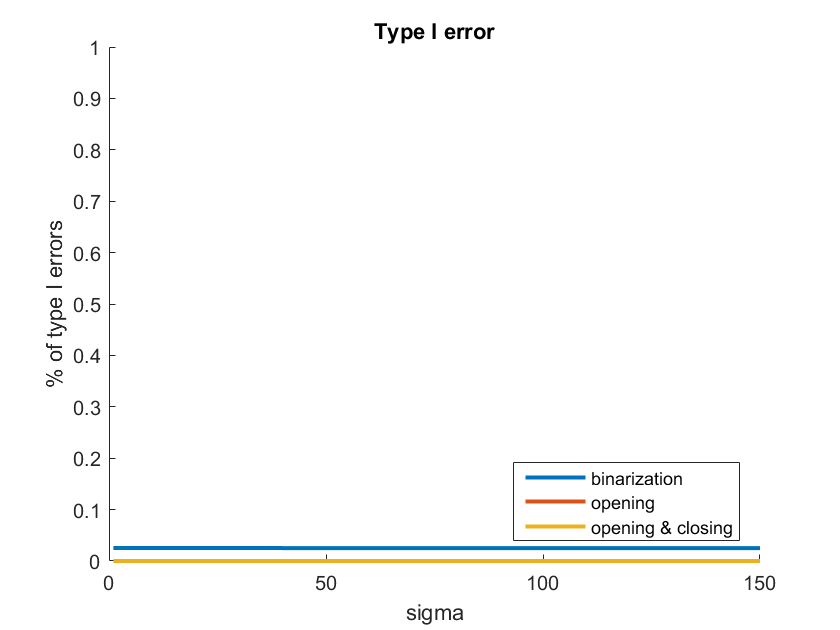
\includegraphics[width=0.6\linewidth]{Morphology/TypeIError}
		\caption[Type I error]{Numerical results of the percentage of type I errors dependent on $\sigma$.}
		\label{fig:TypeIError}
	\end{figure}
\end{frame}

\begin{frame}
	\begin{figure}[h]
		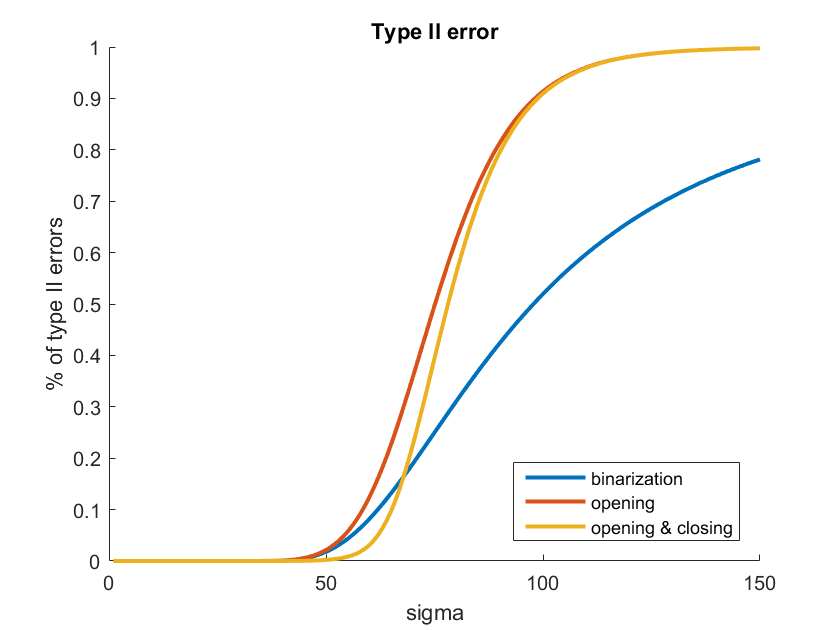
\includegraphics[width=0.6\linewidth]{Morphology/TypeIIError}
		\caption[Type II error]{Numerical results of the percentage of type II errors dependent on $\sigma$.}
		\label{fig:TypeIIError}
	\end{figure}
\end{frame}

%\section{Multiple testing procedures}
%
%\begin{frame}
%	Consider the following setup:
%	\begin{table}[h]
%		\tymax .3\textwidth
%		\begin{tabulary}{\textwidth}{|CCCC|}
%			\hline
%			& \textit{Declared non-significant} & \textit{Declared significant} & \textit{Total} \\
%			\hline
%			\textit{True null hypotheses} & $\mathbf{U}$ & $\mathbf{V}$ & $m_0$ \\
%			\textit{Non-true null hypotheses} & $\mathbf{T}$ & $\mathbf{S}$ & $m - m_0$ \\
%			& $m - \mathbf{R}$ & $\mathbf{R}$ & $m$ \\
%			\hline
%		\end{tabulary}
%	\end{table}
%\end{frame}
%
%\begin{frame}
%	\begin{itemize}
%		\item $m$ is the total number hypotheses tested
%		\item $m_0$ is the number of true null hypotheses, an unknown parameter
%		\item $m - m_0$ is the number of true alternative hypotheses
%		\item $V$ is the number of false positives (Type I error) (also called "false discoveries")
%		\item $S$ is the number of true positives
%		\item $T$ is the number of false negatives (Type II error)
%		\item $U$ is the number of true negatives
%		\item $R = V + S$ is the number of rejected null hypotheses (also called "discoveries", either true or false)
%	\end{itemize}
%	In $m$ hypothesis tests of which $m_0$ are true null hypotheses, $R$ is an observable random variable, and $S$, $T$, $U$, and $V$ are unobservable random variables.
%\end{frame}
%
%\begin{frame}
%	We define another random variable $Q = \frac{V}{V + S}$, which is the proportion of the rejected null hypotheses which are erroneously rejected. We set $Q = 0$, if $V + S = 0$. Based on this, we define the false discovery rate to be
%	\begin{equation*}
%		FDR = \mathbb{E}(Q) = \mathbb{E} \left( \frac{V}{V + S} \right)
%	\end{equation*}
%	
%	We also define the family-wise error rate to be
%	\begin{equation*}
%		FWER = \mathbb{P}( V \geq 1 ) = 1 - \mathbb{P}( V = 0 )
%	\end{equation*}
%	that is the probability of making one or more type I errors.
%\end{frame}
%
%\begin{frame}
%	Three of these multiple testing procedures are given in detail in the following. The first one controls the false discovery rate at level $\alpha$, i.e.
%	\begin{equation*}
%		FDR = \mathbb{E}(Q) \leq \alpha
%	\end{equation*}
%	
%	The other two procedures control the family-wise error rate at level $\alpha$, i.e.
%	\begin{equation*}
%		FWER = \mathbb{P}( V \geq 1 ) \leq \alpha
%	\end{equation*}
%\end{frame}
%
%\begin{frame}
%	First, we calculate for every pixel $(m, n) \in \Omega$ the $p$-value
%	\begin{equation*}
%		p(m, n) = \exp \left( - \frac{\tilde{D}(m, n)^2}{4 \sigma^2} \right) \geq \mathbb{P}(T \geq \tilde{D}(m, n) \mid H_0)
%	\end{equation*}
%\end{frame}
%
%\subsection{FDR Thresholding}
%
%\begin{frame}
%	\begin{itemize}
%		\item Sort $p$-values in ascending order: $p_{(1)} \leq p_{(2)} \leq \dots \leq p_{(M \cdot N)}$
%		\item Calculate the maximal index $k$, such that $p_{(k)} \leq \frac{k \cdot \alpha}{M \cdot N}$
%		\item Calculate the threshold $\lambda_{k} = 2 \sigma \sqrt{- \log(p_{(k)})}$
%		\item Reject all hypotheses $H_{(i)}$ with $p_{(i)} \leq p_{(k)}$, i.e. all hypotheses with $$\tilde{D}_{(i)} \geq \tilde{D}_{(k)} = \lambda_{k} = 2 \sigma \sqrt{- \log(p_{(k)})}$$
%	\end{itemize}
%\end{frame}
%
%\subsection{Bonferroni Thresholding}
%
%\begin{frame}
%	\begin{itemize}
%		\item Reject all hypotheses $H_{i}$ with $p_{i} \leq \frac{\alpha}{M \cdot N}$, i.e. all hypotheses with $$\tilde{D}_{i} \geq \lambda_k = 2 \sigma \sqrt{- \log \left( \frac{\alpha}{M \cdot N} \right)}$$
%	\end{itemize}
%\end{frame}
%
%\subsection{Hochberg Thresholding}
%
%\begin{frame}
%	\begin{itemize}
%		\item Sort $p$-values in ascending order: $p_{(1)} \leq p_{(2)} \leq \dots \leq p_{(M \cdot N)}$
%		\item Calculate the maximal index $k$, such that $p_{(k)} \leq \frac{\alpha}{M \cdot N - k + 1}$
%		\item Reject all hypotheses $H_{(i)}$ with $p_{(i)} \leq p_{(k)}$, i.e. all hypotheses with $$\tilde{D}_{(i)} \geq \tilde{D}_{(k)} = \lambda_{k} = 2 \sigma \sqrt{- \log(p_{(k)})}$$
%	\end{itemize}
%\end{frame}
%
%\begin{frame}
%	All these methods are defined for actual $p$-values, i.e.
%	\begin{equation*}
%		p(m, n) = \mathbb{P}(T \geq \tilde{D}(m, n) \mid H_0)
%	\end{equation*}
%	In contrast to that, we have taken upper bounds for the $p$-values. This is not an issue though, since by taking upper bounds we might decrease the number of hypotheses we reject. Thus it will not increase the error rate.
%	
%	The threshold has the following interpretation:
%	\begin{itemize}
%		\item If $\tilde{D}(m, n) \geq \lambda_{k}$, then $(m, n)$ is part of the ROI.
%		\item If $\tilde{D}(m, n) < \lambda_{k}$, then $(m, n)$ is NOT part of the ROI.
%	\end{itemize}
%\end{frame}


\end{document}
